In this chapter the results for simple observables obtained from the ensembles in \cref{runs:ensembles} are presented. Throughout the chapter, all error estimates associated to expectation values of observables have been computed using the bootstrap method, \cref{app:resampling}, which is a popular resampling method used when the sample size of a statistical population is small, as is our case. The autocorrelation, introduced by the Markov chain, is handled using the procedure found in \cref{app:autocorr} as a correction to the error estimate.

\section{Plaquette and Energy Density} 
The plaquette, \cref{plaquette}, and the energy density, \cref{eq:energy}, are tightly related as they both are estimates of the action. We have already seen in \cref{sec:thermalization} that the plaquette can be used to check whether the metropolis algorithm has thermalized in the early stages of the chain. Another test is to check the dependence of the plaquette on the $\beta$ value of the gluonic action.
\fig[0.7]{results/BetaPlaq.pdf}{Average Plaquette value as a bunction of the inverse coupling $\beta$.}{fig:betplaq}

Since the system is expected, after thermalization, to be at equilibrium,o the sampling of the plaquette and of the energy density should be rather constant in Monte Carlo time. Figure \ref{fig:MCPlaqEnerg} shows that this is indeed the case.
\begin{figure}[hbt!]
    \centering
    \begin{subfigure}{0.45\textwidth}
        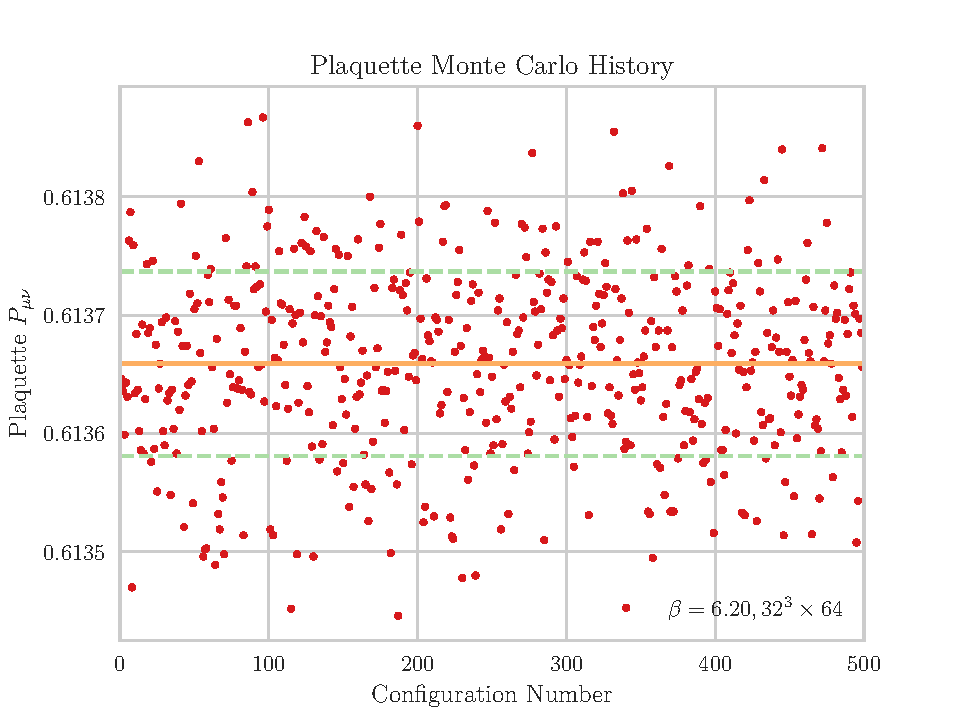
\includegraphics[width=\textwidth]{results/MCPlaq.pdf}
    \end{subfigure}
    \begin{subfigure}{0.45\textwidth}
        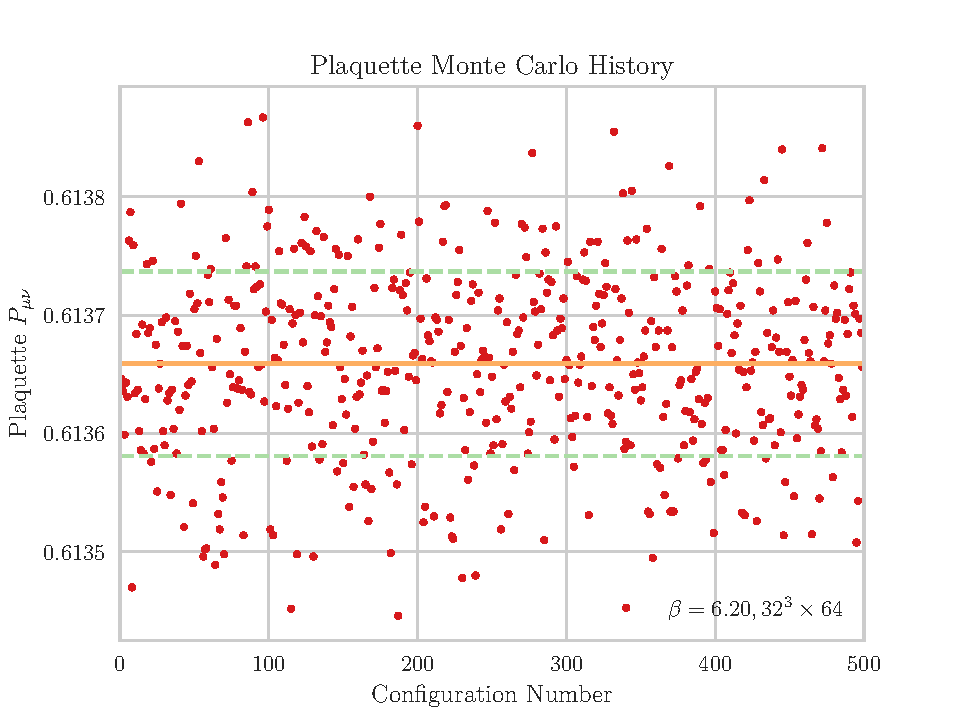
\includegraphics[width=\textwidth]{results/MCPlaq.pdf}
    \end{subfigure}
    \caption{\footnotesize Plaquette and Energy Density as a function of Monte Carlo Time. The blue line is the average and the green dashed lines are the $1\sigma$ interval around it. }
    \label{fig:MCPlaqEnerg}
\end{figure} 

When applying the gradient flow the configuration is evolved towards the minimum of the action, that implies that the values for sufficiently large flow times are both lattice spacing and flow time independent. The results do indeed suggest that this is the case:
\fig[0.7]{results/Plaquette.pdf}{Average plaquette value as a function of flow time $t_f$. }{fig:plaq_plot}
\fig[0.7]{results/Energy.pdf}{Average energy density as a function of flow time $t_f$.}{fig:energy_plot}

Moving to the integrated autocorrelation time for the different ensembles, which we report only for the energy as for the plaquette is almost identical. For all ensembles the value of $\tau_{int}$ never exceeds $1$, meaning that the autocorrelation of the data is not large. Nevertheless, all results of this work (including \cref{fig:plaq_plot} and \cref{fig:energy_plot}) have variances corrected by $\tilde\sigma^2 = 2\tau_{int}\sigma^2$. 
\fig[0.7]{results/EnergyTauInt.pdf}{Integrated autocorrelation time of the Energy Density as a function of flow time. The discontinuity of the data is given by the approximation given by the truncation procedure described in \cref{app:autocorr}}{fig:energyautocorr} 

\section{Topological Charge}
A more interesting quantity to measure is the topological charge. In the continuum it is an integer, with a distribution around zero that resembles a gaussian, though there are studies that prove that indeed it is not a normal distribution \cite{ce_non-gaussianities_2015}. The gradient flow removes the divergencies given by the discretization effect, in \cref{fig:topcsingle} the flow time evolution of three of single configurations is plotted, as an example. We can notice that the value of the topological charge has a plateau at a total smearing of roughly  $0.2$ fm for all cases.  
\fig[0.7]{results/TopcSingle.pdf}{Evolution of the topological charge for three single gauge field configurations, taken at random from the $\beta=6.10$ ensemble.}{fig:topcsingle}
For some configurations however, the plateau is not clear and defined. The explanation could be the too simple definition that has been used for the gauge field strength tensor. Perhaps an improved definition of the tensor, given for example with a linear combination of $1\times 1$, $2\times 1$, $1\times 2$ and $2\times 2$ (or even higher) Wilson Loops could be beneficial.

When taking the average value of the topological charge on all ensembles, we expect the average to be always zero, and from \cref{fig:topc} one can check that our data for the expectation value of $\mathcal{Q}$ is indeed within error-bars always compatible with zero. 
\fig[0.7]{results/TopChar.pdf}{Average topological charge value as a function of flow time $t_f$. Errorbars are computed using bootstrap and corrected with the integrated autocorrelation time.}{fig:topc}

We should note that the increasing error-bars, for $\beta = 6.2$ and $\beta = 6.45$ in particular, are given by the decreasing ensemble size and the increasing autocorrelation time. The integrated autocorrelation time is plotted in \cref{fig:topctauint}, and comparing it with the equivalent plot for the energy density (\cref{fig:energyautocorr}) the difference is clear. The topological charge has a much larger autocorrelation time on the lattice, which grows rapidly with the inverse lattice spacing. It should be noted that the value of $N_{corr}$ is much larger for the $\beta=6.45$ case than all the others, but still the $\tau_{int}$ larger by far.
\fig[0.7]{results/TopcTauInt.pdf}{Integrated autocorrelation time of the topological charge as a function of flow time. The ensembles are the ones reported in \cref{MC:params}, so they have not equal number of cycles between each data point in MC time.}{fig:topctauint}

One last interesting consideration on the topological charge is the distribution of the large flow time value, that is the value it plateaus at. The bins are taken to be centered on integer and half-integer values in order to capture differences of the distribution of the topological charge. On the lattice it can have also not integer values, but from \cref{fig:topchist} it is possible to see that most of the values, especially at large flow time (right histogram), are closer to the integer rather to half-integers.
\begin{figure}[hbt!]
    \centering
    \begin{subfigure}{0.45\textwidth}
        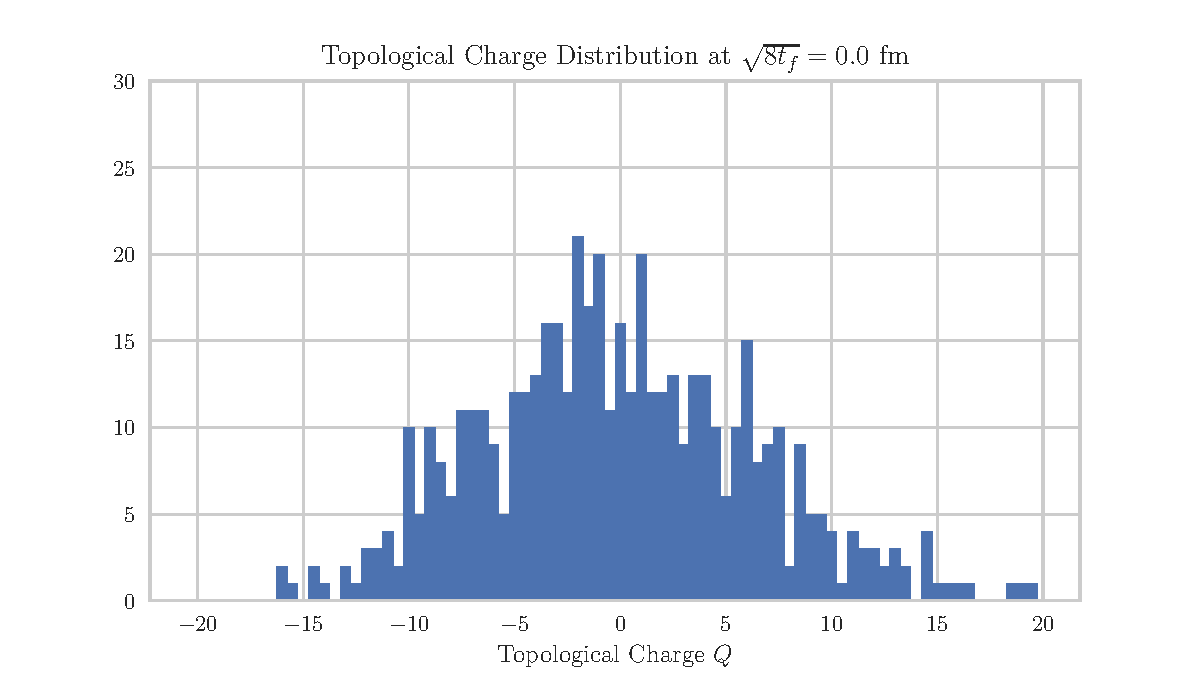
\includegraphics[width=\textwidth]{results/TopcHistNoFlow.pdf}
    \end{subfigure}
    \begin{subfigure}{0.45\textwidth}
        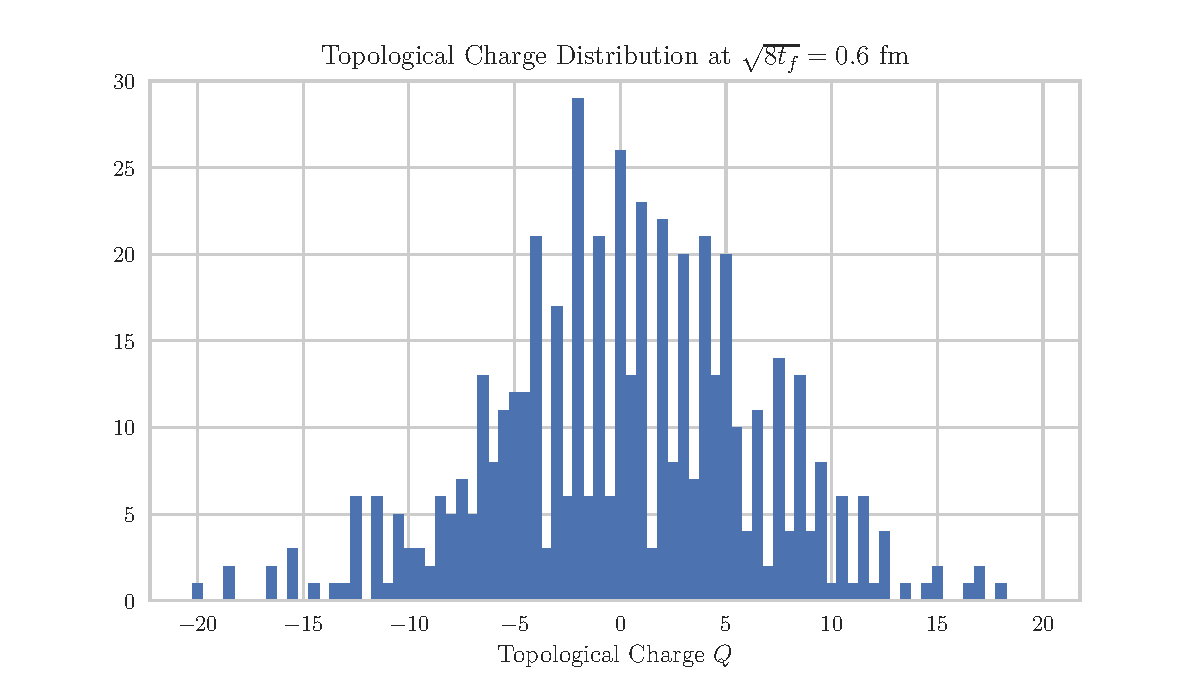
\includegraphics[width=\textwidth]{results/TopcHistFlow.pdf}
    \end{subfigure}
    \caption{\footnotesize Histograms of the topological charge values at $t_f=0$ (left) and $t_f=0.6$ (right) for the $\beta=6.20$ ensemble. The bins are centered on integers and half-integer values.}
    \label{fig:topchist}
\end{figure} 

\section{Topological Susceptiblity}
Another quantity that is interesting to measure is the topological susceptibility. Being the average of the squared topological charge it is related to the width of the distributions in \cref{fig:topchist}. The evolution with the gradient flow of the suceptibility is not trivial. Its value at non-zero flow time does not need renormalization, as for all previously mentioned gluonic observables, but at low flow times the high-frequency fluctuations in the topological charge make it diverge. In order to find the value that effectively reproduces the physical value in the continuum theory one must take the continuum limit. 
\fig[0.7]{results/TopSusc.pdf}{Average topological charge value as a function of flow time $t_f$. Errorbars are computed using bootstrap and corrected with the integrated autocorrelation time.}{fig:tops} 

Here we can see the value of $\chi^{\frac{1}{4}} = \langle Q^2 \rangle ^{\frac{1}{4}}$ which in physical units is an energy hence reported in MeV. We notice the fluctuations for low flow times are removed by the gradient flow. It is then possible to take the continuum limit in a region between $0.4$ fm and $0.6$ fm. 
The behavior at zero flow time is not what we were expecting, comparing for example to \cite{shindler_nucleon_2015} we don't observe a clear divergency at $\sqrt{8t_f} = 0$. The behavior seems to be more more divergent (a true divergency is impossible, it is always a finite quantity on the lattice) for larger values of $\beta$. This could be due to the usage of the clover definition of the gauge field strength tensor, one of the differences between this work and the reference, that perhaps removes low distance noise from the lattice, which contributes to an oversampling of the low topological charge values. This behavior should be investigated \NOTE{SHOULD I REF MATHIAS'S WORK?}.\\
When taking the continuum limit we recover the following value, taken by considering the value of the susceptibility around $\sqrt{8t_f} = 0.5$:
\beq
    \chi^{\frac{1}{4}} = 186.9(4.9)~\text{MeV} 
    \label{val:tops}
\eeq 
This is compatible with the value in \cite{shindler_nucleon_2015} of  $\chi^{\frac{1}{4}}_{ref} = 195.9(4.9)~\text{MeV} $.
\fig[0.7]{results/TopsContLimit.pdf}{Continuum limit extrapolation of $\chi^{\frac{1}{4}}$. The black point is the extrapolated point.}{fig:topscontlimit}
As an additional result we can use this extrapolation to compute the mass of the $\eta'$ meson taken from the Witten-Veneziano formula:
\beq
    \chi = \frac{F_\pi^2m_{\eta'}^2}{2N_{flavors}}
\eeq 
Using as inputs $F_\pi = 92$ MeV, the pion decay constant, and having $N_{flavors} = 3$ naturally, the $\eta'$ mass is:
\beq    
    m^{(lattice)}_{\eta'} = \sqrt{\frac{\chi^{\frac{1}{4}} 2N_{flavors}}{F_\pi^2}} = 921(16)~\text{MeV} 
\eeq
which we compare with an experimental value  $m^{(exp)}_{\eta'} = 957.78(6)$ MeV, so we are off by more than $2\sigma$, but probably the result is largely influenced by the data point obtained from $\beta=6.45$, which has less statistics (only 250 configurations) and larger uncertainty.